\chapter{Smart Grid}\label{chap:sg}
The Smart Grid  is a new concept of grid which introduces new technologies into the common power system. They enable power grids to become more efficient, integrate other sources of energy than traditional ones, such as renewable energies, and increase the overall management performance by using modern information technologies. The SG is capable of delivering power in more efficient way and respond to a wide ranging condition an events \cite{journals/comsur/FangMXY12}. 
There are several definitions for the SG among the literature. For example \cite{journals/comsur/FangMXY12} states that  "\textit{SG can be regarded as an electric system that uses information, two-way and cyber-secure communication technologies and computational intelligence in a integrated fashion to achieve a clean, safe, secure, reliable, resilient, efficient and sustainable system}".\cite{conf/isgt/GhoshPR13} considers the SG as "\textit{a platform that embraces several multidisciplinary concepts towards computerization of electrical power grids}". The common concept over the literature is that SG main goal is to integrate several components, traditional and new, to achieve better performance, interoperability, energy management and sustainability in long term. \\
SG creates an environment that introduces a converge between the infrastructure of generation, transmission, distribution, energy, information technology and digital communication infrastructure that enables the exchange of information and control action among the various segments of the power grid.\\
As is it possible to notice, these integration means that the SG itself is a very complicated system. Achieving the mentioned goals is a complex task. Due to is variety of problems and challenges, most of the proposed solution and studies regarding the SG focus in some specific aspects. 
An interesting table that presents a comparison between the traditional grid and the SG is presented in \cite{journals/comsur/FangMXY12}:
\begin{figure}[h]
\centering
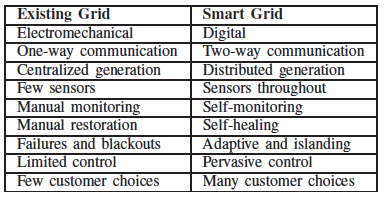
\includegraphics[width=0.5\textwidth]{/Users/rafaelremondes/UM/MEI/Thesis/DistributedAggregationAlgortihmsSM/Writing/Images/differencesTraditionalSmart}
\caption{\label{fig:comparisonOldNew} Brief Comparison Between the Existing Grid and the Smar Grid}
\end{figure}

\section{Smart Grid Model}
 The components in a traditional grid go one way, contrary to what happens in SG where all the flows of electricity and information goes two-way.  So the role of each component are quite different, for example, a consumer can both consume energy from the grid and provide it too considering that he has a device that produces renewable energy. A specific component of grid, such as household, can both receive energy from the global grid and in the next moment, can disconnect from it and become self-sustainable. The NIST report \cite{government2011nist} proposes a conceptual model providing the main actors towards the SG.
\begin{figure}[h]
\centering
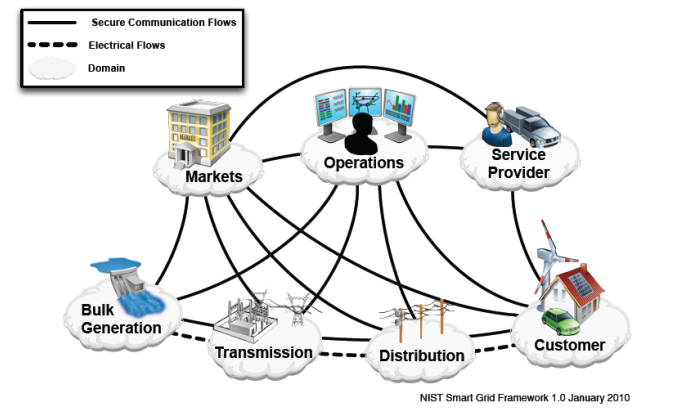
\includegraphics[width=0.75\textwidth]{/Users/rafaelremondes/UM/MEI/Thesis/DistributedAggregationAlgortihmsSM/Writing/Images/NIST_model}
\caption{\label{fig:NIST_model} NIST Conceptual Model for SG}
\end{figure}
Costumers, the end users of electricity, Markets, Service Providers, Electricity Companies, Operations, Managers of the Movement of electricity, Bulk Generation, Generation Centers, Transmission and Distribution of energy. 
In \cite{journals/comsur/FangMXY12} it is provided a more technical approach where the SG is separated into three major subsystems:
\begin{itemize}
\item \textit{Smart infrastructure system} embraces the energy subsytem, information subsystem and communication infrastructure subsystem. The energy subsystem is responsible for advanced electricity generation, delivery and consumption. The information subsystems are responsible for information metering, monitoring and management in the context of the SG. Finally, the communication subsystem is responsible for the communication among the various components and also its connectivity.   
\item \textit{Smart management system} Provides advanced management and control services and functionalities, \cite{journals/comsur/FangMXY12} considers this system the key reason why SG can revolutionize the grid.  Most of the new grid goals are related to energy efficiency improvement, supply and demand balance, emission control etc. and it is the scope of problems the management systems tries to resolve.
\item \textit{Smart protection system} Provides advanced grid reliability analysis, failure protection, security and privacy protection services.
 \end{itemize}
We will take a more precise look in the smart information subsystem, where is the aim of this work considering it involves the AMR. We are interested in the measurement data that comes from the smart meters. The next section details the SG information subsystem.

\section{Smart Information SubSystem}
This part of the SG refers to all the information that is collected by sensing the consumer consumption and its management . The data collected is often used for billing, grid status monitoring and user appliance control \cite{journals/comsur/FangMXY12}. Then, it is aggregated and \textit{smart management} is ideally performed on it.\\
An important concept in the information subsystem  is the \textit{Smart Metering} and the Smart Metering System or Automatic Meter Reading \nom{AMR}{Automatic Meter Reading}. This system is responsible for collect the data from the measurments that are performed by the SMs.\\
Other part of the Smart Information SubSystem is the \textit{Smart Monitoring and Measurement} which can be approached by either \textit{sensors} or \textit{phasor measurement units}(PMU). \textit{Sensors} are used for detecting failures, tower collapses, hotspots and extreme mechanical conditions. They can also provide real-time diagnose of the grid status. PMU's are devices that measures the electrical waves on a electrical grid to determinate the health  of the system.
The management refers to all the information analysis and modeling, integration and optimization.\\
In this specific part of SG there are several areas of research that represent a new set of opportunities.


\section{Smart Grid Communication}
The most important question in the communication is "\textit{ what network and communication should be used}"\cite{journals/comsur/FangMXY12}? Since there is no standard communication system in SG, several solutions were proposed.The solutions can be grouped into two types: wired communications and wireless communications. Wired communication are harder to implement than wireless ones because of the need to deploy them from zero and also due to the costs involved in installing non-existing cables to provide the communication. For that reasons, wired communication are more expensive.  Wireless communication are a better option considering the costs, time to deploy and furthermore they are normally more suitable for remote end applications \cite{parikh2010opportunities}. However, they lack some performance compared to wired solutions.\\
There are several wireless possibilities for communication.\\
\begin{itemize}
  \item \textit{Wireless Mesh Network} (WMN) is a communication network made up for radio nodes organized in a mesh topology\cite{journals/comsur/FangMXY12}. Increases reliability and automatic network connectivity, has large coverage and high data rate.
\item \textit{Cellular Communication Systems}  GSM and 3G. Useful in case of low computation power devices such as the meters. It it quick and low-cost to obtain data communications coverage over a large geographic area \cite{akyol2010survey}. There several solutions that uses a Short Message Service communication to send the meters data.
\item \textit{Wireless Communication based on 802.15.4} ZigBee is a wireless communication that is recommended to be used in SG considering the IEEE 802.15.4 protocol stack\cite{parikh2010opportunities}. ZigBee is designed for radio-frequency applications that require low data rate, long battery life, and secure networking. Selected as the communication technology for the smart metering devices\cite{farhangi2010path} because it provides a standardized platform for exchanging data between smart metering devices and appliances located on costumer  premises\cite{journals/comsur/FangMXY12}. However, ZigBee is not suitable for long distances, unlike, for example, WiMax. WirelessHART and ISA100.11a are other examples of wireless communications based on the IEEE 802.15.4 protocol.
\end{itemize}
Other examples of wireless communication are stallite communication, cognitive radio and  microwave communications.
Fiber-optic Communications and Power-line Communications are some of the wired communication possibilities. Power-line communication has the advantage of been already installed, so the cost of deployment is way less than other wired solution, but has also big security disadvantages. Fiber-Optic has the advantage of being fast and more secure but is very expensive to deploy.\\



%%%%%SMART METERS-----------------%

\section{Smart Meters}
Smart meters are devices that sense the energy consumption. They are installed in the costumer side,  households orin  industrial facilities, depending on the costumer nature Playing a major role in the information subsystem, smart meters present several number of challenges in sensing, analyzing, and communication\cite{journals/spm/ErkinTLP13}. SMs, more specifically, the Smart Mettering System has also the denomination of AMR(Automatic Meter Reading). In \cite{khalifa2011survey} the AMR is referred as the technology whose goal is to help collect the meter measurement automatically and possibly send commands to the meters.\\
As referred, the main function of a smart meter, and all meters, is sense the consumption in the costumer side. Plus that, this smart devices also have communication capabilities. So, every pre-defined period of time, they communicate the sensed consumption to a central device that aggregates the collected data. This feature, allows a company to remotely read the consumers' consumption at each household, without the need to actually go to the premises and without notifying the costumers\cite{Ericsson_2}. Jorge Vasconcelos \cite{RePEc:erp:euirsc:p0193} enlightens in his work the potential benefits of the smart meters, for  example, the potential benefits for customers are customer awareness and energy saving, more accurate meter reading, billing, better service quality, greater tariff variety and flexibility, improved conditions for vulnerable customers, easier comparability of offers and it is easier to change supplier. \cite{khalifa2011survey} states some benefits of the smart metering system: Real time pricing, power quality measurement, automated Billing, Load management,, Remote Connect/Disconnect, Outage notification and Bundling with water and gas.\\
Privacy and security are important concerns when dealing with the sensed information. There are many privacy issues considering that external parties access the consumer energy consumption. Some are authorized parties, but there is a risk of an unauthorized access of this data, leaving to some security and privacy dangers. For example, by analyzing the data, one could determinate which devices are plugged in at some specific time, giving for example information about if there is people in home or note. Many works propose solution to securely store this sensible information. Although privacy and security are out of the scope of this work, it is important to mention this point.\\
The smart meters, as any desirable component of the SG, enable two way communication. The two-way communication will be dissecated in \ref{subsec:amrami} .

\subsection{AMR and AMI}\label{subsec:amrami}
As referred in this document, the smart metering system, i.e., the system of smart meters that sense the energy consumption and send it to a Gateway or a Data Collector, is mentioned as an AMR. In \cite{journals/spm/ErkinTLP13} the definition of an AMR is described in more detail as an "\textit{technology of automatically collecting diagnostic, consumption and status data from energy metering devices and transferring that data to a database for billing troubleshooting and analyzing}".
The Automated Metering Infrastructure \nom{AMI}{Automated Metering Infrastructure} differs from the traditional AMR because it provides two-way communication, enabling a more sophisticated control of a smart meter behavior. Therefore, all of a meter information is available in real time, allowing improved system operations and  costumer power demand management\cite{journals/spm/ErkinTLP13}.  AMI has also the ability of reconfigure from communication failures, perform outage management and reporting, service connect and disconnect and also enables time stamping of meter data \cite{hart2008using}. AMI are built upon AMR. 
In this work, we are only interested in collected information from the smart meters about the consumption, however, two-way communication is an important feature that should be considered. First, most benefits of smart meters come from two-way communication. Second two-way communication are not important only for behavior control and outage detection, it enables the realization and implementation of in-network algorithms. The communication flow collector-smart meter enable, for example, the \textit{request} phase, which are part of many algorithms.\\
In this document, when referring to AMR, it is referring to an AMR that has an AMI built upon it enabling two-way communication. 
